% !TeX program = lualatex
% ================================================================
% Polish Parallel Text Version of SolvingEquationsStarters
%
% Generated by the server using the following settings:
%
%   language            Polish (pol)
%   text direction      left to right
%   font                Noto Serif
%   fallback font       Noto Serif
%   built from          latex/starters/retrieval/KS3/solvingEquationsStarters.tex
%   vocabulary key      latex/starters/retrieval/KS3/solvingEquationsStarters/L2/pol/solvingEquationsStarters_polishKey.tex
%   tier 3 vocabulary   green   RGB 0 128 0
%   English text        black   RGB 0 0 0
%   Polish text         purple  RGB 112 48 160
%   layout macros       version 3
%   sheet layout        version 1
%
% Please don't edit any information in this comment block - the server
% compares it against the current settings and rebuilds this file when
% they differ, so changes here would be overwritten. However, feel free
% to make updates to the LaTeX below if you want to edit it.
% ================================================================

\documentclass{beamer}
% ================================================================
% Copied from the English sheet this was translated from, so that
% anything it sets up for itself still works here
% ================================================================
\usepackage{tikz}
\usetikzlibrary{calc, arrows.meta, decorations.pathreplacing}
\usepackage{pgfplots}
\pgfplotsset{compat=1.18}
\usepackage{multicol}
\usepackage{amsmath}
\usepackage{amssymb}

% ================================================================
% Retrieval starters for a Year 8 top set, used across the solving
% equations unit.
%
% Every starter draws on each of the four earlier topics: fractions,
% decimals and percentages; percentages with multipliers, including
% simple and compound interest; money problems, best buys and currency
% conversion, including conversion graphs; and the laws of indices,
% including fractions and decimals as the base with negative integer
% indices. Each starter uses more of the equations unit than the one
% before, in the order it is taught:
%
%   1  missing-number problems in words, such as "what number multiplied
%      by 7 makes 21?", answered by reasoning, with one written as an
%      equation; and, separately, the algebraic manipulation the unit
%      needs: collecting like terms, the index laws, expanding brackets
%      and substituting. No equation is solved formally on this starter.
%   2  one- and two-step equations, solved by doing the same thing to both
%      sides. A reverse percentage and a conversion graph read backwards
%      are one-step equations.
%   3  the unknown on both sides, and with brackets. A bar model that
%      takes the same amount from both sides, two simple interest
%      accounts on a graph, and a recurring decimal as an equation.
%   4  the unknown in the denominator: multiply both sides by it. The
%      price per roll in a best buy, a bill shared equally, and
%      x^-1 = 1/x.
%   5  equations with algebraic fractions. A car that loses a quarter of
%      its value each year, and a fraction-of-an-amount problem on a bar
%      model split into twelfths.
%   6  simultaneous equations. Two receipts, simple interest from a
%      table, two bureaux de change, and the index laws.
%
% Every starter has equations for pupils to form from a context. There
% are no quadratic equations.
%
% The methods follow the ones the class was taught:
%   - Equations are solved by doing the same thing to both sides, never
%     with a flow chart. The working is set out with the operation written
%     under both sides. Starter 2 gives the operations, starter 4 gives the
%     new one (multiplying both sides by the unknown), and starter 5 leaves
%     them blank.
%   - Compound interest and compound decrease are shown with flow charts.
%     Interest is never shown with a bar model.
%   - Division by a decimal is done with equivalent fractions, for
%     example 36 / 0.8 = 360 / 8 = 45.
%   - A decimal base is written as a simplified fraction before a
%     negative index is used, and a negative index turns the fraction
%     upside down.
%   - A recurring decimal is turned into a fraction by the algebraic
%     method only.
%
% The questions are worded as briefly as possible. Within each starter
% they run from retrieval of the earlier topics to the new idea, and the
% last question on each starter is a challenge.
% ================================================================

\setbeamertemplate{navigation symbols}{}
\setbeamersize{text margin left=0.4cm, text margin right=0.4cm}
\setlength{\multicolsep}{3pt}
\setlength{\columnsep}{16pt}

% ================================================================
% Answer-overlay helpers
% ================================================================
\newcommand{\ablank}[1]{%
  \alt<2>{\textcolor{red}{#1}}{\underline{\phantom{#1}}}%
}
\newcommand{\ashow}[1]{\uncover<2->{\textcolor{red}{\small #1}}}
\newcommand{\ashowq}[1]{\alt<2->{\textcolor{red}{\small #1}}{?}}

% Answers drawn straight on to a TikZ diagram, revealed on overlay 2 like \ashow.
% Space is reserved on overlay 1, so the diagram does not move between slides.
\usetikzlibrary{overlay-beamer-styles}
\tikzset{
  ans/.style     = {red, thick, visible on=<2->},
  ansfill/.style = {red!15, visible on=<2->},
  anslab/.style  = {red, font=\tiny, visible on=<2->},
}

% Used by the worked solutions rather than by this deck, so that each worked
% solution is first a question with room to write in and then the answer.
\newlength{\aworkpad}
\setlength{\aworkpad}{8mm}
\newcommand{\awork}[1]{%
  \par\vspace{\aworkpad}%
  \uncover<2->{#1}%
  \par\vspace{\aworkpad}%
}

% Every question list on these slides is tight, so that the diagram column and
% the question column both finish inside the slide.
\newcommand{\tightlist}{%
  \setlength{\itemsep}{0pt}\setlength{\parskip}{0pt}\setlength{\topsep}{0pt}%
}

% ================================================================
% The pictures these starters are built from.
% ================================================================
\tikzset{
  dhead/.style  = {font=\scriptsize\bfseries, anchor=west},
  vans/.style   = {anslab, font=\scriptsize},
  brace/.style  = {decorate, decoration={brace, amplitude=3pt}},
  mbrace/.style = {decorate, decoration={brace, mirror, amplitude=3pt}},
  bcell/.style  = {draw, fill=blue!6},
  bpart/.style  = {draw, fill=orange!12},
}

% Solving an equation by doing the same thing to both sides. The lines of the
% equation are lined up on the equals sign. Between two lines, \bsop writes the
% operation under both sides, and \bsopgap leaves it as a blank to fill in.
%   \begin{bothsides}{Working for Q4}
%     4x-7 & = & 29\\  \bsop{+7}  4x & = & \ablank{36}\\ ...
%   \end{bothsides}
\newenvironment{bothsides}[1]
  {\par{\scriptsize\bfseries #1}\par\vspace{0.1em}\footnotesize
   \hspace*{0.5cm}$\renewcommand{\arraystretch}{1.15}\begin{array}{@{}r@{\;}c@{\;}l@{}}}
  {\end{array}$\par}
\newcommand{\bsopstyle}[1]{\text{\scriptsize\color{blue!55!black}$#1$}}
\newcommand{\bsop}[1]{\bsopstyle{#1} & & \bsopstyle{#1}\\}
\newcommand{\bsopgap}[1]{\text{\scriptsize\ablank{$#1$}} & & \text{\scriptsize\ablank{$#1$}}\\}

% Flow charts, for compound interest and compound decrease only. The chain runs
% forwards along the top, with one multiplier on each arrow. \flowback draws the
% way back underneath, from right to left, with a division on each arrow. The
% arrow labels have a fixed height, so that an answer revealed on an arrow does
% not move the rest of the slide.
\tikzset{
  fbox/.style   = {draw, rounded corners=2pt, minimum width=0.9cm,
                   inner sep=1pt, font=\footnotesize, text height=2.2ex, text depth=0.9ex},
  farrow/.style = {-{Stealth[length=4pt]}, thick},
  barrow/.style = {-{Stealth[length=4pt]}, thick, gray!70!black, bend left=40},
  flab/.style   = {font=\scriptsize, inner sep=1.5pt, text height=1.6ex, text depth=0.5ex},
}
% \flowchart{name}{box 1}{op 1}{box 2}{op 2}{box 3}
\newcommand{\flowchart}[6]{%
  \node[fbox] (#1a) at (0.45,0) {#2};
  \node[fbox] (#1b) at (2.1,0)  {#4};
  \node[fbox] (#1c) at (3.75,0) {#6};
  \draw[farrow] (#1a) -- node[flab, above] {#3} (#1b);
  \draw[farrow] (#1b) -- node[flab, above] {#5} (#1c);
}
% \flowback{name}{back op 2}{back op 1}
\newcommand{\flowback}[3]{%
  \draw[barrow] (#1c.south) to node[flab, below] {#2} (#1b.south);
  \draw[barrow] (#1b.south) to node[flab, below] {#3} (#1a.south);
}

% Graphs: a light grid, small tick labels, and the axis labels pulled in
% close so that the graph fits the diagram column.
\pgfplotsset{
  startergraph/.style = {
    scale only axis, width=3.2cm,
    grid=both, grid style={black!12}, axis lines=left,
    tick label style={font=\tiny}, label style={font=\scriptsize},
    xlabel style={yshift=4pt}, ylabel style={yshift=-6pt},
  },
}

% A receipt from a café, drawn with a torn bottom edge.
% \receipt{x}{first line}{second line}{total}, with its top-left corner at (x,0)
\newcommand{\receipt}[4]{%
  \draw[fill=yellow!4, draw=black!60]
    (#1,0) -- ({#1+1.95},0) -- ({#1+1.95},-1.3)
    \foreach \i in {1,...,6} { -- ({#1+1.95-0.325*\i+0.1625},-1.38) -- ({#1+1.95-0.325*\i},-1.3) }
    -- cycle;
  \node[anchor=west] at ({#1+0.1},-0.25) {#2};
  \node[anchor=west] at ({#1+0.1},-0.58) {#3};
  \draw[black!50, dashed] ({#1+0.1},-0.8) -- ({#1+1.85},-0.8);
  \node[anchor=west, font=\scriptsize\bfseries] at ({#1+0.1},-1.05) {Total};
  \node[anchor=east] at ({#1+1.85},-1.05) {#4};
}

\title{Solving Equations: Starters}
\author{}
\date{}

% Characters this language's font has not got are borrowed from another,
% rather than being silently dropped - see docs/translated-sheet-latex.md
\directlua{%
  if luaotfload and luaotfload.add_fallback then
    luaotfload.add_fallback("eallatinfallback",
      { "Noto Serif:mode=harf;" })
  else
    tex.error("this luaotfload is too old to register a fallback font")
  end
}
\usepackage[english]{babel}
\babelprovide[import]{polish}
\babelfont[polish]{rm}[Renderer=Harfbuzz, BoldFont={Noto Serif}, ItalicFont={Noto Serif}, BoldItalicFont={Noto Serif}, RawFeature={fallback=eallatinfallback}]{Noto Serif}
\babelfont[polish]{sf}[Renderer=Harfbuzz, BoldFont={Noto Serif}, ItalicFont={Noto Serif}, BoldItalicFont={Noto Serif}, RawFeature={fallback=eallatinfallback}]{Noto Serif}
\newcommand{\ealtext}[1]{\foreignlanguage{polish}{#1}}
\newcommand{\ealtextblock}[1]{{\raggedright\foreignlanguage{polish}{#1}\par}}
% ================================================================
% EAL layout helpers
% ================================================================
\usepackage{xcolor}

\definecolor{ealkeycolour}{RGB}{0,128,0}
\definecolor{ealenglish}{RGB}{0,0,0}
\definecolor{ealtwocolour}{RGB}{112,48,160}

\newsavebox{\ealboxen}
\newsavebox{\ealboxtr}
\newlength{\ealglosswd}
\newlength{\ealglossraise}
\setlength{\ealglossraise}{1.15em}

% a tier 3 word, in English and in translation alike
\newcommand{\ealkey}[1]{\textcolor{ealkeycolour}{#1}}
\newcommand{\ealkeytr}[1]{\textcolor{ealkeycolour}{\ealtext{#1}}}

% One translated word above one English word. Built from kernel
% primitives, never a tabular, which would break wherever the sheet
% loads array, booktabs or tabularx. The box is as wide as the wider of
% the two, so a long translation pushes its neighbours aside instead of
% overlapping them, and it claims its full height so a table row or a
% TikZ node makes room for it.
\newcommand{\ealgloss}[2]{%
  \sbox{\ealboxen}{\ealkey{#1}}%
  \sbox{\ealboxtr}{\small\textcolor{ealtwocolour}{\ealtext{#2}}}%
  \setlength{\ealglosswd}{\wd\ealboxen}%
  \ifdim\wd\ealboxtr>\ealglosswd\setlength{\ealglosswd}{\wd\ealboxtr}\fi
  \leavevmode
  \makebox[\ealglosswd][c]{%
    \makebox[0pt][c]{\usebox{\ealboxen}}%
    \makebox[0pt][c]{\raisebox{\ealglossraise}{\usebox{\ealboxtr}}}%
  }%
}

% opens up line spacing around a block of glosses, so the raised
% translations sit clear of the line above
\newenvironment{ealglossed}{\par\linespread{2.1}\selectfont\ignorespaces}{\par}

% a whole translated sentence above its English counterpart. block level,
% so it does not belong inside a tabular cell
\newcommand{\ealpara}[2]{%
  \par\addvspace{0.5\baselineskip}%
  {\color{ealtwocolour}\ealtextblock{#1}}%
  \penalty200
  {\color{ealenglish}#2\par}%
  \addvspace{0.5\baselineskip}%
}

\begin{document}

\frame{\titlepage}

%------------------------------------------------------------------
% STARTER 1
%------------------------------------------------------------------
\begin{frame}[t]{Starter 1: Missing Numbers \& \ealkey{Expressions} (1 of 3)}
\begin{center}
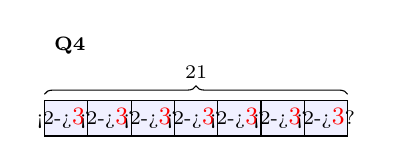
\begin{tikzpicture}[every node/.style={font=\scriptsize}]
\node[dhead] at (0,1.15) {Q4};
\begin{scope}[x=0.55cm]
\foreach \i in {0,...,6} {
  \draw[bcell] (\i,0) rectangle ({\i+1},0.45);
  \node at ({\i+0.5},0.225) {\ashowq{3}};}
\draw[brace] (0,0.53) -- (7,0.53) node[midway, above=2pt] {$21$};
\end{scope}
\end{tikzpicture}
\end{center}
\footnotesize
\begin{enumerate}\tightlist
\setcounter{enumi}{0}
\item \ealpara{$\tfrac25=$}{$\tfrac25=$ \ablank{$40\%$}}
\item \ealpara{$3^{-2}$}{$3^{-2}$ \ashow{$=\tfrac19$}}
\item \ealpara{$0.2^{-1}$}{$0.2^{-1}$ \ashow{$=\left(\tfrac15\right)^{-1}=5$}}
\item \ealpara{Jaka liczba pomnożona przez $7$ daje $21$?}{What number multiplied by $7$ makes $21$? \ashow{$3$}}
\item \ealpara{Jaka liczba plus $8$ daje $3$?}{What number plus $8$ makes $3$? \ashow{$-5$}}
\end{enumerate}
\end{frame}

\begin{frame}[t]{Starter 1: Missing Numbers \& \ealkey{Expressions} (2 of 3)}
\footnotesize
\begin{enumerate}\tightlist
\setcounter{enumi}{5}
\item \ealpara{Jaka liczba pomnożona przez $1.2$ daje $60$?}{What number multiplied by $1.2$ makes $60$? \ashow{$\tfrac{60}{1.2}=\tfrac{600}{12}=50$}}
\item \ealpara{Ile biletów po \pounds1.50 można kupić za \pounds12?}{How many \pounds1.50 tickets can \pounds12 buy? \ashow{$\tfrac{12}{1.5}=\tfrac{120}{15}=8$}}
\item[] \ealpara{Uprość \ealkeytr{wyrażenia} poniżej:}{\ealkey{Simplify} the \ealkey{expressions} below:}
\item \ealpara{$3a+5b-a+2b$}{$3a+5b-a+2b$ \ashow{$2a+7b$}}
\item \ealpara{$2a\times3a^4$}{$2a\times3a^4$ \ashow{$6a^5$}}
\end{enumerate}
\end{frame}

\begin{frame}[t]{Starter 1: Missing Numbers \& \ealkey{Expressions} (3 of 3)}
\ealpara{Siatka do Q10}{Grid for Q10}
\begin{center}
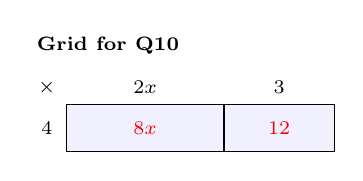
\begin{tikzpicture}[every node/.style={font=\scriptsize}]
\begin{scope}[yshift=-1.55cm]
\node[dhead] at (0,0.75) {Grid for Q10};
\node at (0.25,0.22) {$\times$};
\node at (1.5,0.22)  {$2x$};
\node at (3.2,0.22)  {$3$};
\node at (0.25,-0.3) {$4$};
\draw[bcell] (0.5,-0.6) rectangle (2.5,0);
\draw[bcell] (2.5,-0.6) rectangle (3.9,0);
\node[vans] at (1.5,-0.3) {$8x$};
\node[vans] at (3.2,-0.3) {$12$};
\end{scope}
\end{tikzpicture}
\end{center}
\footnotesize
\begin{enumerate}\tightlist
\setcounter{enumi}{9}
\item \ealpara{\ealkeytr{Wymnóż nawiasy} w $4(2x+3)$, używając siatki.}{\ealkey{Expand} $4(2x+3)$ using the grid. \ashow{$8x+12$}}
\item \ealpara{\ealkeytr{Wymnóż nawiasy} i \ealkeytr{uprość} $3(x+2)-2(x-1)$.}{\ealkey{Expand} and \ealkey{simplify} $3(x+2)-2(x-1)$. \ashow{$3x+6-2x+2=x+8$}}
\item \ealpara{Oblicz $5-3x$, gdy $x=-2$.}{Find $5-3x$ when $x=-2$. \ashow{$5-3\times(-2)=11$}}
\item \ealpara{(Wyzwanie) Pomyśl o liczbie, podwój ją i dodaj $6$. Podziel wynik na pół, a następnie odejmij liczbę, od której zacząłeś. Pokaż za pomocą \ealkeytr{algebry}, że zawsze otrzymujesz $3$.}{(Challenge) Think of a number, double it and add $6$. Halve the result, then subtract the number you started with. Show with \ealkey{algebra} that you always get $3$. \ashow{$\tfrac{2x+6}{2}-x=x+3-x=3$}}
\end{enumerate}
\end{frame}

%------------------------------------------------------------------
% STARTER 2
%------------------------------------------------------------------
\begin{frame}[t]{Starter 2: One- \& Two-Step \ealkey{Equations} (1 of 3)}
\ealpara{Obliczenia do Q4}{Working for Q4}
\begin{bothsides}{Working for Q4}
  4x-7 & = & 29\\
  \bsop{+7}
  4x   & = & \ablank{36}\\
  \bsop{\div4}
  x    & = & \ablank{9}
\end{bothsides}
\footnotesize
\begin{enumerate}\tightlist
\setcounter{enumi}{0}
\item \ealpara{$\tfrac38=$}{$\tfrac38=$ \ablank{$37.5$}$\%$}
\item \ealpara{$2^{-3}$}{$2^{-3}$ \ashow{$=\tfrac18$}}
\item \ealpara{$0.5^{-2}$}{$0.5^{-2}$ \ashow{$=\left(\tfrac12\right)^{-2}=2^2=4$}}
\item \ealpara{Myślę o liczbie $x$, mnożę ją przez $4$ i odejmuję $7$, aby otrzymać $29$. Zapisz \ealkeytr{równanie}, a następnie uzupełnij obliczenia po lewej.}{I think of a number $x$, multiply it by $4$ and subtract $7$ to get $29$. Write an \ealkey{equation}, then complete the working on the left. \ashow{$4x-7=29$}}
\end{enumerate}
\end{frame}

\begin{frame}[t]{Starter 2: One- \& Two-Step \ealkey{Equations} (2 of 3)}
\footnotesize
\begin{enumerate}\tightlist
\setcounter{enumi}{4}
\item[] \ealpara{Rozwiąż każde \ealkeytr{równanie}.}{Solve each \ealkey{equation}.}
\item \ealpara{$3x+5=26$}{$3x+5=26$ \ashow{$3x=21$, \; $x=7$}}
\item \ealpara{$7-2x=15$}{$7-2x=15$ \ashow{$-2x=8$, \; $x=-4$}}
\item \ealpara{Uzupełnij zdanie: obniżka o $20\%$ pozostawia $80\%$ pierwotnej kwoty. Aby znaleźć kwotę po obniżce, mnożymy kwotę pierwotną przez ...}{Complete the sentence: a reduction by $20\%$ leaves $80\%$ of the original amount. To find the amount after the reduction we multiply the original by \ablank{$0.8$}.}
\item \ealpara{Cena spada o $20\%$ do \pounds36. \ealkeytr{Rozwiąż} \ealkeytr{równanie}, aby znaleźć cenę pierwotną, \pounds$p$.}{A price falls by $20\%$ to \pounds36. \ealkey{Solve} an \ealkey{equation} to find the original price, \pounds$p$. \ashow{$0.8p=36$, \; $p=\tfrac{36}{0.8}=\tfrac{360}{8}=45$}}
\end{enumerate}
\end{frame}

\begin{frame}[t]{Starter 2: One- \& Two-Step \ealkey{Equations} (3 of 3)}
\ealpara{\pounds? przy \ealkeytr{procencie składanym} $10\%$}{\pounds? at $10\%$ \ealkey{compound interest}}
\begin{center}
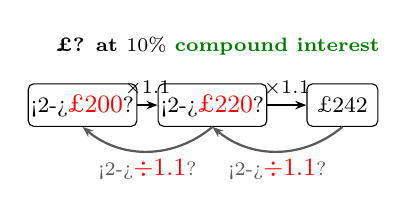
\begin{tikzpicture}[every node/.style={font=\scriptsize}]
\node[dhead] at (0,0.75) {\pounds? at $10\%$ \ealkey{compound interest}};
\flowchart{b}{\ashowq{\pounds200}}{$\times1.1$}{\ashowq{\pounds220}}{$\times1.1$}{\pounds242}
\flowback{b}{\ashowq{$\div1.1$}}{\ashowq{$\div1.1$}}
\end{tikzpicture}
\end{center}
\ealpara{Wykres przeliczeniowy}{Conversion graph}
\begin{center}
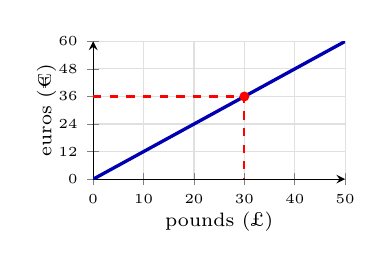
\begin{tikzpicture}
\begin{axis}[startergraph, height=1.75cm,
  xmin=0, xmax=50, ymin=0, ymax=60,
  xtick={0,10,...,50}, ytick={0,12,...,60},
  xlabel={pounds (\pounds)}, ylabel={euros (\texteuro)},
]
  \addplot[blue!70!black, very thick, domain=0:50] {1.2*x};
  \draw[ans, dashed] (axis cs:0,36) -- (axis cs:30,36) -- (axis cs:30,0);
  \fill[ans] (axis cs:30,36) circle (1.8pt);
\end{axis}
\end{tikzpicture}
\end{center}
\footnotesize
\begin{enumerate}\tightlist
\setcounter{enumi}{8}
\item \ealpara{Uzupełnij schemat. Ile zainwestowano?}{Complete the flow chart. How much was invested? \ashow{$\tfrac{242}{1.1}=\tfrac{2420}{11}=220$, \; $\tfrac{2200}{11}=200$}}
\item \ealpara{Użyj wykresu, aby zamienić \texteuro36 na funty. Sprawdź, \ealkeytr{rozwiązując} $1.2x=36$.}{Use the graph to change \texteuro36 into pounds. Check by \ealkey{solving} $1.2x=36$. \ashow{\pounds30; \; $x=\tfrac{360}{12}=30$}}
\item \ealpara{(Wyzwanie) \ealkeytr{Rozwiąż} $2^{x+4}=\tfrac18$.}{(Challenge) \ealkey{Solve} $2^{x+4}=\tfrac18$. \ashow{$2^{x+4}=2^{-3}$, \; $x+4=-3$, \; $x=-7$}}
\end{enumerate}
\end{frame}

%------------------------------------------------------------------
% STARTER 3
%------------------------------------------------------------------
\begin{frame}[t]{Starter 3: \ealkey{Unknowns} on \ealkey{Both Sides} (1 of 3)}
\ealpara{\ealkeytr{Model słupkowy} do Q3}{\ealkey{Bar model} for Q3}
\begin{center}
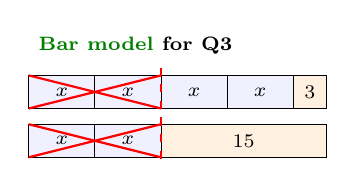
\begin{tikzpicture}[every node/.style={font=\scriptsize}]
\node[dhead] at (0,0.8) {\ealkey{Bar model} for Q3};
\begin{scope}[x=0.14cm]
\foreach \i in {0,...,3} {
  \draw[bcell] ({6*\i},0) rectangle ({6*\i+6},0.42);
  \node at ({6*\i+3},0.21) {$x$};}
\draw[bpart] (24,0) rectangle (27,0.42);
\node at (25.5,0.21) {$3$};
\foreach \i in {0,1} {
  \draw[bcell] ({6*\i},-0.62) rectangle ({6*\i+6},-0.2);
  \node at ({6*\i+3},-0.41) {$x$};}
\draw[bpart] (12,-0.62) rectangle (27,-0.2);
\node at (19.5,-0.41) {$15$};
\foreach \y in {0,-0.62} {
  \draw[ans] (0,\y) -- (12,{\y+0.42});
  \draw[ans] (0,{\y+0.42}) -- (12,\y);}
\draw[ans, dashed] (12,0.52) -- (12,-0.72);
\end{scope}
\end{tikzpicture}
\end{center}
\footnotesize
\begin{enumerate}\tightlist
\setcounter{enumi}{0}
\item \ealpara{Czym jest $0.45$ jako \ealkeytr{ułamek}?}{What is $0.45$ as a \ealkey{fraction}? \ashow{$\tfrac{45}{100}=\tfrac{9}{20}$}}
\item \ealpara{\ealkeytr{Uprość} $3x^{-2}\times4x^5$}{\ealkey{Simplify} $3x^{-2}\times4x^5$ \ashow{$12x^3$}}
\item \ealpara{Użyj \ealkeytr{modelu słupkowego}, aby \ealkeytr{rozwiązać} $4x+3=2x+15$.}{Use the \ealkey{bar model} to \ealkey{solve} $4x+3=2x+15$. \ashow{Take $2x$ from \ealkey{both sides}: \; $2x+3=15$, \; $x=6$}}
\item[] \ealpara{Rozwiąż każde \ealkeytr{równanie}.}{Solve each \ealkey{equation}.}
\item \ealpara{$7x-4=3x+24$}{$7x-4=3x+24$ \ashow{$4x-4=24$, \; $x=7$}}
\end{enumerate}
\end{frame}

\begin{frame}[t]{Starter 3: \ealkey{Unknowns} on \ealkey{Both Sides} (2 of 3)}
\ealpara{Wykres dla Q6 i Q7}{Graph for Q6 and Q7}
\begin{center}
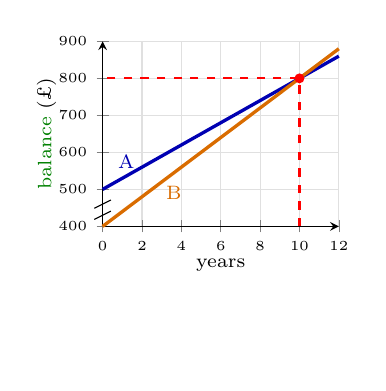
\begin{tikzpicture}
\begin{axis}[startergraph, width=3.0cm, height=2.35cm,
  xmin=0, xmax=12, ymin=400, ymax=900,
  xtick={0,2,...,12}, ytick={400,500,...,900},
  xlabel={years}, ylabel={\ealkey{balance} (\pounds)}, clip=false,
]
  \fill[white] ($(rel axis cs:0,0.06)+(-3pt,0)$) rectangle ($(rel axis cs:0,0.12)+(3pt,0)$);
  \draw ($(rel axis cs:0,0.06)+(-3pt,-1.5pt)$) -- ++(6pt,3pt);
  \draw ($(rel axis cs:0,0.12)+(-3pt,-1.5pt)$) -- ++(6pt,3pt);
  \addplot[blue!70!black, very thick, domain=0:12] {500+30*x}
    node[pos=0.1, above, font=\scriptsize, inner sep=2pt] {A};
  \addplot[orange!85!black, very thick, domain=0:12] {400+40*x}
    node[pos=0.25, below right, font=\scriptsize, inner sep=1pt] {B};
  \draw[ans, dashed] (axis cs:10,400) -- (axis cs:10,800) -- (axis cs:0,800);
  \fill[ans] (axis cs:10,800) circle (1.8pt);
\end{axis}
\end{tikzpicture}
\end{center}
\footnotesize
\begin{enumerate}\tightlist
\setcounter{enumi}{4}
\item \ealpara{$6(x-2)=2x+8$}{$6(x-2)=2x+8$ \ashow{$6x-12=2x+8$, \; $x=5$}}
\item \ealpara{A ma \pounds500 przy $6\%$, a B ma \pounds400 przy \ealkeytr{procencie prostym} $10\%$ rocznie. Zapisz \ealkeytr{saldo} każdego po $n$ latach.}{A has \pounds500 at $6\%$ and B has \pounds400 at $10\%$ \ealkey{simple interest} a year. Write each \ealkey{balance} after $n$ years. \ashow{A: $500+30n$, \; B: $400+40n$}}
\item \ealpara{Kiedy \ealkeytr{salda} są równe? \ealkeytr{Rozwiąż} \ealkeytr{równanie}, a następnie sprawdź na wykresie.}{When are the \ealkey{balances} equal? \ealkey{Solve} an \ealkey{equation}, then check on the graph. \ashow{$500+30n=400+40n$, \; $100=10n$, \; $n=10$}}
\end{enumerate}
\end{frame}

\begin{frame}[t]{Starter 3: \ealkey{Unknowns} on \ealkey{Both Sides} (3 of 3)}
\footnotesize
\begin{enumerate}\tightlist
\setcounter{enumi}{7}
\item \ealpara{\ealkeytr{Rozwiąż} $7^{3x}=7^{x+8}$}{\ealkey{Solve} $7^{3x}=7^{x+8}$ \ashow{$3x=x+8$, \; $x=4$}}
\item \ealpara{Ile to \pounds250 w euro, przy \texteuro1.16 za \pounds1?}{What is \pounds250 in euros, at \texteuro1.16 per \pounds1 \ashow{\texteuro290}}
\item \ealpara{(Wyzwanie) $x=0.\dot7$. Użyj $10x-x$, aby zapisać $x$ jako \ealkeytr{ułamek}.}{(Challenge) $x=0.\dot7$. Use $10x-x$ to write $x$ as a \ealkey{fraction}. \ashow{$10x=7.\dot7$, \; $9x=7$, \; $x=\tfrac79$}}
\end{enumerate}
\end{frame}

%------------------------------------------------------------------
% STARTER 4
%------------------------------------------------------------------
\begin{frame}[t]{Starter 4: \ealkey{Unknown} in the \ealkey{Denominator} (1 of 3)}
\ealpara{Bułki. Tabela: Paczka, Bułki, Cena, Cena za bułkę}{Bread rolls. Table: Pack, Rolls, Price, Per roll}
\begin{center}
{\scriptsize
\renewcommand{\arraystretch}{1.4}\setlength{\tabcolsep}{3.5pt}
\begin{tabular}{c|c|c|c}
  Pack & Rolls & Price & Per roll\\ \hline
  A & $4$ & \pounds1.60 & \ablank{$40$p}\\
  B & $6$ & \pounds2.10 & \ablank{$35$p}\\
  C & $n$ & \pounds3.60 & $30$p
\end{tabular}}
\end{center}
\footnotesize
\begin{enumerate}\tightlist
\setcounter{enumi}{0}
\item \ealpara{$\tfrac{7}{20}=$}{$\tfrac{7}{20}=$ \ablank{$35$}$\%$}
\item \ealpara{$0.4^{-2}$}{$0.4^{-2}$ \ashow{$=\left(\tfrac25\right)^{-2}=\left(\tfrac52\right)^2=\tfrac{25}{4}$}}
\item \ealpara{Uzupełnij tabelę. Który zakup jest korzystniejszy, A czy B?}{Complete the table. Which is the better buy, A or B? \ashow{B}}
\item \ealpara{\ealkeytr{Rozwiąż} \ealkeytr{równanie}, aby znaleźć $n$ dla paczki C.}{\ealkey{Solve} an \ealkey{equation} to find $n$ for pack C. \ashow{$\tfrac{360}{n}=30$, \; $360=30n$, \; $n=12$}}
\end{enumerate}
\end{frame}

\begin{frame}[t]{Starter 4: \ealkey{Unknown} in the \ealkey{Denominator} (2 of 3)}
\ealpara{Obliczenia do Q5}{Working for Q5}
\begin{bothsides}{Working for Q5}
  \dfrac{12}{x} & = & 3\\
  \bsop{\times x}
  12 & = & \ablank{3x}\\
  \bsop{\div3}
  \ablank{4} & = & x
\end{bothsides}
\footnotesize
\begin{enumerate}\tightlist
\setcounter{enumi}{4}
\item[] \ealpara{Rozwiąż każde \ealkeytr{równanie}.}{Solve each \ealkey{equation}.}
\item \ealpara{$\dfrac{12}{x}=3$}{$\dfrac{12}{x}=3$ \ashow{$x=4$}}
\item \ealpara{$\dfrac{35}{x-2}=5$}{$\dfrac{35}{x-2}=5$ \ashow{$35=5(x-2)$, \; $x=9$}}
\item \ealpara{$3+\dfrac{18}{x}=9$}{$3+\dfrac{18}{x}=9$ \ashow{$\tfrac{18}{x}=6$, \; $x=3$}}
\end{enumerate}
\end{frame}

\begin{frame}[t]{Starter 4: \ealkey{Unknown} in the \ealkey{Denominator} (3 of 3)}
\ealpara{Rachunek do Q8}{The bill for Q8}
\begin{center}
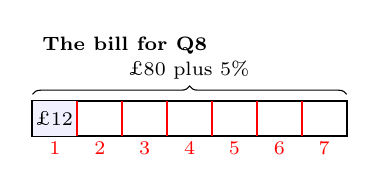
\begin{tikzpicture}[every node/.style={font=\scriptsize}]
\node[dhead] at (0,1.15) {The bill for Q8};
\begin{scope}[x=0.57cm]
\draw[thick] (0,0) rectangle (7,0.45);
\draw[bcell] (0,0) rectangle (1,0.45);
\node at (0.5,0.225) {\pounds12};
\draw[brace] (0,0.53) -- (7,0.53) node[midway, above=2pt] {\pounds80 plus $5\%$};
\foreach \i in {1,...,6} \draw[ans] (\i,0) -- (\i,0.45);
\foreach \i in {1,...,7} \node[vans, below, inner sep=2pt] at ({\i-0.5},0) {\i};
\end{scope}
\end{tikzpicture}
\end{center}
\footnotesize
\begin{enumerate}\tightlist
\setcounter{enumi}{7}
\item \ealpara{Rachunek na \pounds80 ma doliczone $5\%$ za obsługę i jest dzielony równo po \pounds12 na osobę. \ealkeytr{Rozwiąż} \ealkeytr{równanie}, aby znaleźć liczbę osób, $p$.}{A \pounds80 bill has $5\%$ service added, and is split equally at \pounds12 each. \ealkey{Solve} an \ealkey{equation} to find the number of people, $p$. \ashow{$\tfrac{84}{p}=12$, \; $84=12p$, \; $p=7$}}
\item \ealpara{\ealkeytr{Rozwiąż} $5x^{-1}=20$.}{\ealkey{Solve} $5x^{-1}=20$. \ashow{$\tfrac5x=20$, \; $5=20x$, \; $x=\tfrac14$}}
\item \ealpara{(Wyzwanie) \ealkeytr{Rozwiąż} $\dfrac{50}{x+2}=0.8^{-2}$.}{(Challenge) \ealkey{Solve} $\dfrac{50}{x+2}=0.8^{-2}$. \ashow{$\left(\tfrac45\right)^{-2}=\tfrac{25}{16}$, \; $800=25(x+2)$, \; $x=30$}}
\end{enumerate}
\end{frame}

%------------------------------------------------------------------
% STARTER 5
%------------------------------------------------------------------
\begin{frame}[t]{Starter 5: \ealkey{Equations} with \ealkey{Fractions} (1 of 3)}
\ealpara{Obliczenia do Q3}{Working for Q3}
\begin{bothsides}{Working for Q3}
  \dfrac{x+2}{3} & = & 5\\
  \bsopgap{\times3}
  x+2 & = & \ablank{15}\\
  \bsopgap{-2}
  x   & = & \ablank{13}
\end{bothsides}
\footnotesize
\begin{enumerate}\tightlist
\setcounter{enumi}{0}
\item \ealpara{$\tfrac13+\tfrac14$}{$\tfrac13+\tfrac14$ \ashow{$=\tfrac{7}{12}$}}
\item \ealpara{$\left(\tfrac34\right)^{-2}$}{$\left(\tfrac34\right)^{-2}$ \ashow{$=\left(\tfrac43\right)^2=\tfrac{16}{9}$}}
\item[] \ealpara{Rozwiąż każde \ealkeytr{równanie}.}{Solve each \ealkey{equation}.}
\item \ealpara{$\dfrac{x+2}{3}=5$}{$\dfrac{x+2}{3}=5$ \ashow{$x=13$}}
\item \ealpara{$\dfrac{2x-1}{5}=3$}{$\dfrac{2x-1}{5}=3$ \ashow{$2x-1=15$, \; $x=8$}}
\end{enumerate}
\end{frame}

\begin{frame}[t]{Starter 5: \ealkey{Equations} with \ealkey{Fractions} (2 of 3)}
\ealpara{Wartość samochodu w \pounds, w ciągu $2$ lat}{A car's value in \pounds, over $2$ years}
\begin{center}
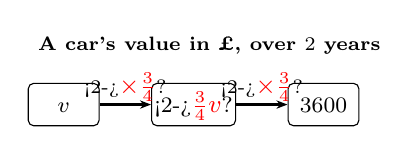
\begin{tikzpicture}[every node/.style={font=\scriptsize}]
\node[dhead] at (0,0.75) {A car's value in \pounds, over $2$ years};
\flowchart{c}{$v$}{\ashowq{$\times\tfrac34$}}{\ashowq{$\tfrac34v$}}%
  {\ashowq{$\times\tfrac34$}}{$3600$}
\end{tikzpicture}
\end{center}
\footnotesize
\begin{enumerate}\tightlist
\setcounter{enumi}{4}
\item \ealpara{$\dfrac{x}{3}+\dfrac{x}{4}=14$}{$\dfrac{x}{3}+\dfrac{x}{4}=14$ \ashow{$4x+3x=168$, \; $x=24$}}
\item \ealpara{$\dfrac{x+3}{2}=\dfrac{x+7}{3}$}{$\dfrac{x+3}{2}=\dfrac{x+7}{3}$ \ashow{$3(x+3)=2(x+7)$, \; $x=5$}}
\item \ealpara{Samochód traci $25\%$ swojej wartości każdego roku. Uzupełnij schemat, a następnie \ealkeytr{rozwiąż} \ealkeytr{równanie} dla $v$.}{A car loses $25\%$ of its value each year. Complete the flow chart, then \ealkey{solve} an \ealkey{equation} for $v$. \ashow{$\tfrac{9}{16}v=3600$, \; $9v=57\,600$, \; $v=6400$}}
\end{enumerate}
\end{frame}

\begin{frame}[t]{Starter 5: \ealkey{Equations} with \ealkey{Fractions} (3 of 3)}
\ealpara{Pieniądze Sama}{Sam's money}
\ealpara{$5$ części to \pounds15, więc $1$ część to \pounds3}{$5$ parts are \pounds15, so $1$ part is \pounds3}
\begin{center}
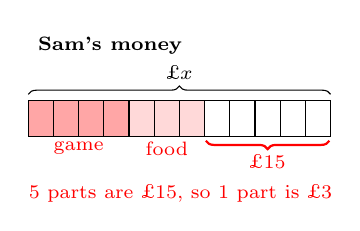
\begin{tikzpicture}[every node/.style={font=\scriptsize}]
\node[dhead] at (0,1.15) {Sam's money};
\begin{scope}[x=0.32cm]
\fill[ansfill, red!35] (0,0) rectangle (4,0.45);
\fill[ansfill, red!15] (4,0) rectangle (7,0.45);
\foreach \i in {0,...,11} \draw ({\i},0) rectangle ({\i+1},0.45);
\draw[brace] (0,0.53) -- (12,0.53) node[midway, above=2pt] {\pounds$x$};
\node[vans, below, inner sep=2pt] at (2,0) {game};
\node[vans, below, inner sep=2pt] at (5.5,0) {food};
\draw[ans, mbrace] (7.05,-0.06) -- (11.95,-0.06);
\node[vans, below, inner sep=2pt] at (9.5,-0.16) {\pounds15};
\node[vans, anchor=north west, inner sep=0pt] at (0,-0.62)
  {$5$ parts are \pounds15, so $1$ part is \pounds3};
\end{scope}
\end{tikzpicture}
\end{center}
\footnotesize
\begin{enumerate}\tightlist
\setcounter{enumi}{7}
\item \ealpara{Sam ma \pounds$x$. Wydaje $\frac13$ na grę i $\frac14$ na jedzenie, zostaje mu \pounds15. Zaznacz na pasku, a następnie \ealkeytr{rozwiąż} \ealkeytr{równanie} dla $x$.}{Sam has \pounds$x$. He spends $\frac13$ on a game and $\frac14$ on food, leaving \pounds15. Shade the bar, then \ealkey{solve} an \ealkey{equation} for $x$. \ashow{$x-\tfrac{x}{3}-\tfrac{x}{4}=15$, \; $\tfrac{5x}{12}=15$, \; $x=36$}}
\item \ealpara{\ealkeytr{Rozwiąż} $\left(\dfrac23\right)^{x}=\dfrac94$.}{\ealkey{Solve} $\left(\dfrac23\right)^{x}=\dfrac94$. \ashow{$\left(\tfrac23\right)^{-2}=\tfrac94$, \; so $x=-2$}}
\item \ealpara{(Wyzwanie) \pounds3 kupuje $x$ bułek, a \pounds4 kupuje $x+4$ bułek, w tej samej cenie za bułkę. Znajdź $x$.}{(Challenge) \pounds3 buys $x$ rolls and \pounds4 buys $x+4$ rolls, at the same price per roll. Find $x$. \ashow{$\tfrac{3}{x}=\tfrac{4}{x+4}$, \; $3(x+4)=4x$, \; $x=12$}}
\end{enumerate}
\end{frame}

%------------------------------------------------------------------
% STARTER 6
%------------------------------------------------------------------
\begin{frame}[t]{Starter 6: \ealkey{Simultaneous Equations} (1 of 3)}
\ealpara{Dwa rachunki: $2$ kawy i $3$ ciasta = \pounds9.30; $2$ kawy i $1$ ciasto = \pounds5.50}{Two receipts: $2$ coffees, $3$ cakes = \pounds9.30; $2$ coffees, $1$ cake = \pounds5.50}
\begin{center}
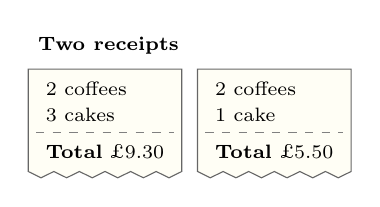
\begin{tikzpicture}[every node/.style={font=\scriptsize}]
\node[dhead] at (0,0.3) {Two receipts};
\receipt{0}{$2$ coffees}{$3$ cakes}{\pounds9.30}
\receipt{2.15}{$2$ coffees}{$1$ cake}{\pounds5.50}
\end{tikzpicture}
\end{center}
\footnotesize
\begin{enumerate}\tightlist
\setcounter{enumi}{0}
\item \ealpara{$0.125$ jako \ealkeytr{ułamek}}{$0.125$ as a \ealkey{fraction} \ashow{$\tfrac18$}}
\item \ealpara{$2^{-1}+2^{-2}$ jako \ealkeytr{procent}}{$2^{-1}+2^{-2}$ as a \ealkey{percentage} \ashow{$\tfrac12+\tfrac14=75\%$}}
\item \ealpara{Zapisz każdy rachunek jako \ealkeytr{równanie}, gdzie $c$ oznacza kawę, a $k$ ciasto. Odejmij, aby znaleźć $k$ i $c$.}{Write each receipt as an \ealkey{equation}, with $c$ for a coffee and $k$ for a cake. Subtract to find $k$ and $c$. \ashow{$2c+3k=9.30$, \; $2c+k=5.50$; \; $2k=3.80$, \; $k=1.90$, \; $c=1.80$}}
\end{enumerate}
\end{frame}

\begin{frame}[t]{Starter 6: \ealkey{Simultaneous Equations} (2 of 3)}
\ealpara{\pounds$P$ przy \pounds$I$ \ealkeytr{procencie prostym} rocznie. Tabela: Lata, \ealkeytr{saldo}}{\pounds$P$ at \pounds$I$ \ealkey{simple interest} a year. Table: Years, \ealkey{balance}}
\begin{center}
{\scriptsize
\renewcommand{\arraystretch}{1.3}
\begin{tabular}{l|c|c}
  Years   & $2$        & $5$\\ \hline
  \ealkey{Balance} & \pounds560 & \pounds650
\end{tabular}}
\end{center}
\footnotesize
\begin{enumerate}\tightlist
\setcounter{enumi}{3}
\item[] \ealpara{Rozwiąż każdą parę \ealkeytr{równań}.}{Solve each pair of \ealkey{equations}.}
\item \ealpara{$\begin{aligned}[t] x+y&=10\\ x-y&=4 \end{aligned}$}{$\begin{aligned}[t] x+y&=10\\ x-y&=4 \end{aligned}$ \ashow{$x=7$, \; $y=3$}}
\item \ealpara{$\begin{aligned}[t] 2x+3y&=13\\ x+y&=5 \end{aligned}$}{$\begin{aligned}[t] 2x+3y&=13\\ x+y&=5 \end{aligned}$ \ashow{$x=2$, \; $y=3$}}
\item \ealpara{Zapisz dwa \ealkeytr{równania} z tabeli i \ealkeytr{rozwiąż} je. Znajdź \ealkeytr{stopę procentową}.}{Write two \ealkey{equations} from the table, and \ealkey{solve} them. Find the \ealkey{interest rate}. \ashow{$P+2I=560$, \; $P+5I=650$; \; $I=30$, \; $P=500$; \; $6\%$}}
\end{enumerate}
\end{frame}

\begin{frame}[t]{Starter 6: \ealkey{Simultaneous Equations} (3 of 3)}
\ealpara{Lotnisko: bez opłaty, i \texteuro1.10 za każde \pounds1. High Street: opłata \pounds5, potem \texteuro1.20 za każde pozostałe \pounds1.}{Airport: no fee, and \texteuro1.10 for every \pounds1. High Street: a \pounds5 fee, then \texteuro1.20 for every \pounds1 that is left.}
\parbox{\linewidth}{\raggedright\scriptsize
  \textbf{Airport}: no fee, and \texteuro1.10 for every \pounds1.\\[2pt]
  \textbf{High Street}: a \pounds5 fee, then \texteuro1.20 for every \pounds1 that is left.}
\footnotesize
\begin{enumerate}\tightlist
\setcounter{enumi}{6}
\item \ealpara{Zapisz kwotę w euro, $y$, którą każde biuro wymienia za \pounds$x$. Kiedy są równe?}{Write the euros, $y$, that each bureau gives for \pounds$x$. When are they equal? \ashow{$y=1.1x$, \; $y=1.2x-6$; \; $0.1x=6$, \; $x=\tfrac{6}{0.1}=\tfrac{60}{1}=60$}}
\item \ealpara{(Wyzwanie) \ealkeytr{Rozwiąż} $2^x\times2^y=64$ i $3^x\div3^y=\tfrac19$.}{(Challenge) \ealkey{Solve} $2^x\times2^y=64$ and $3^x\div3^y=\tfrac19$. \ashow{$x+y=6$, \; $x-y=-2$; \; $x=2$, \; $y=4$}}
\end{enumerate}
\end{frame}

\end{document}